%Die Angabe des schlauen Spruchs auf diesem Wege funtioniert nur,
%wenn keine Änderung des Kapitels mittels den in preambel/chapterheads.tex
%vorgeschlagenen Möglichkeiten durchgeführt wurde.
%\setchapterpreamble[u]{%
%\dictum[Albert Einstein]{Probleme kann man niemals mit derselben Denkweise lösen, durch die sie entstanden sind.}
%}

\chapter{Ergebnisse und Resultate}
\label{chap:results}

Durch diese Arbeit konnte insbesondere durch die Erweiterung durch den räumlichen Glattheitsterm und die Ergänzung mit subquadratischen Bestrafungstermen eine Verbesserung der Ergebnisse festegestellt werden.
Die Implementierung des Standard-Verfahrens von Debevec und Malik zeigt insbesondere bei der Generierung der Antwortkurve aus allen Bildpunkten Probleme mit der Glattheit der Antwortkurve auf (siehe \autoref{fig:res:1}). Der Vergleich zur herkömmlichen Methode, bei der nur eine begrenzte Anzahl an Bildpunkten verwendet wird, zeigt jedoch wenig Unterschiede in der Antwortkurve.

In den nachfolgenden Beschreibungen werden folgende Symbole mit den angegebenen Standardwerten verwendet, falls nichts anderes dazu angegeben wird:
\begin{description}
\item[$\lambda$]: Gewicht des Glattheitsterms für $\b g$, Standard: 50
\item[$\mu$]: Gewicht der Monotonie-Beschränkung für $\b g$, Standard: 0
\item[$\alpha$]: Gewicht der räumlichen Glattheit für $\b E$, Standard: 0
\item[$\#$]: Anzahl der Iterationen beim iterativen Lösen, Standard: 10
\item[$\sigma$]: Standardabweichung des additiven Gauss-Rauschen, Standard: 0
\end{description}


\begin{figure}
  \begin{center}
    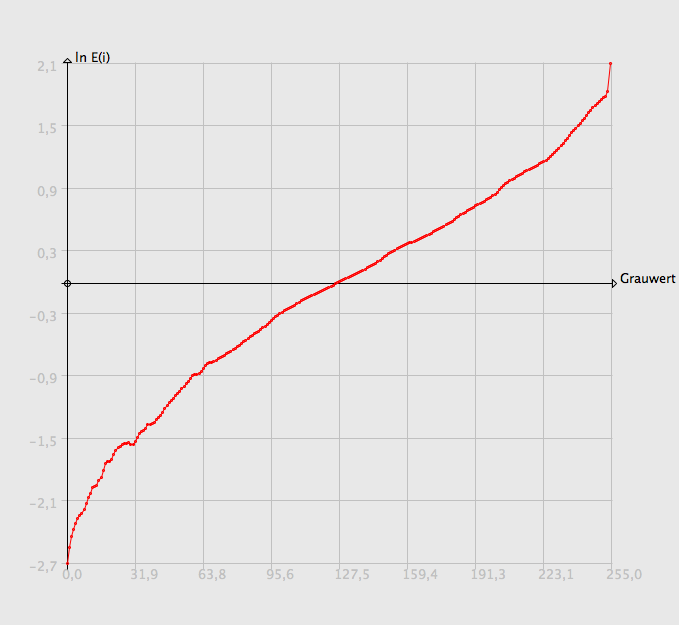
\includegraphics[height=5cm, width=6cm]{results/g1}
    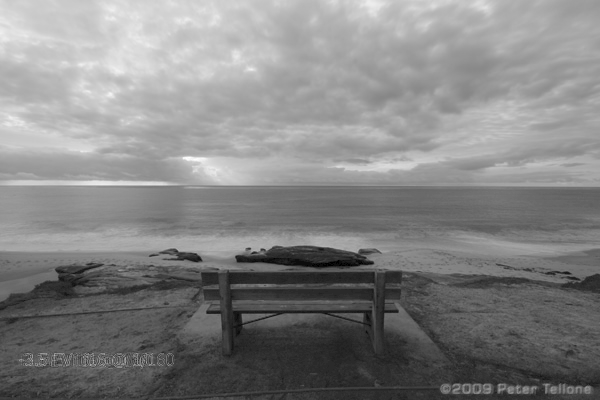
\includegraphics[height=5cm]{results/E1}
    \\ \vspace{5pt}
    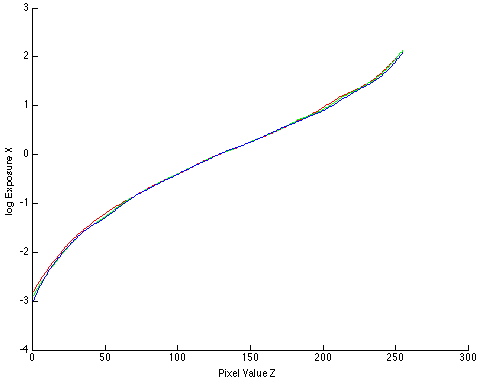
\includegraphics[height=5cm, width=6cm]{results/g1_external}
    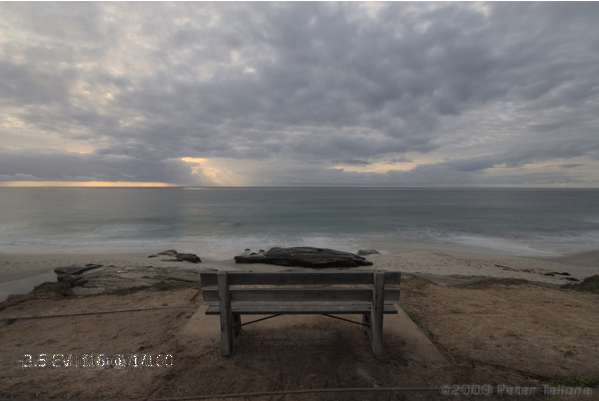
\includegraphics[height=5cm]{results/E1_external}
    \caption{Verfahren der Berechnung der Antwortkurve (li.) und dem dazugehörigen Resultat (re.) \textbf{oben:} Unser Verfahren, \textbf{unten:} Implementierung von Mathias Eitz, siehe \autoref{sec:implementations}  (keine Erweiterungen aktiviert)}
    \label{fig:res:1}
  \end{center}
\end{figure}

\section{Ergebnisse mit Erweiterungen}
Die in dieser Arbeit vorgestellten Erweiterungen sollen die Resultate noch weiter verbessern. Dazu werden Stück für Stück die Veränderungen in der Antwortkurve gezeigt.

\subsection{Ergebnisse mit \gls{Monotonie}-Bedingung}

Bei den meisten Bildern ist die Antwortkurve $\b g$ bereits von sich aus monoton steigend. Um eine Bildserie zu erhalten, bei der die Kurve diese Eigenschaft nicht bereits durch das Standard-Verfahren erhält, wurden eigene Bilder aufgenommen (siehe \autoref{fig:mon:1}). Diese Belichtungsserie liefert zunächst eine recht unförmige Antwortkurve, welche auch durch mehr Iterationen nicht weiter konvergiert. Durch die Erweiterung der Monotonie kann die Kurve entsprechend begradigt und verbessert werden.

\begin{figure}
  \begin{center}
    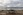
\includegraphics[width=0.3\textwidth]{sample_2/1}
    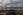
\includegraphics[width=0.3\textwidth]{sample_2/2}
    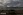
\includegraphics[width=0.3\textwidth]{sample_2/3}\\ \vspace{5pt}
    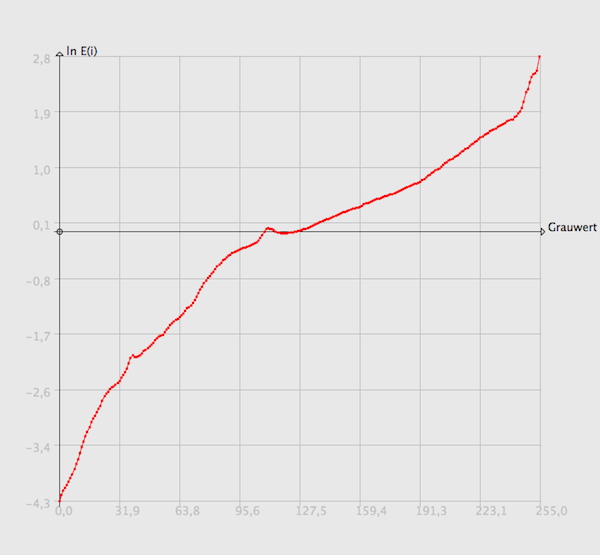
\includegraphics[width=0.45\textwidth]{sample_2/g_no_mon} \hspace{1pt}
    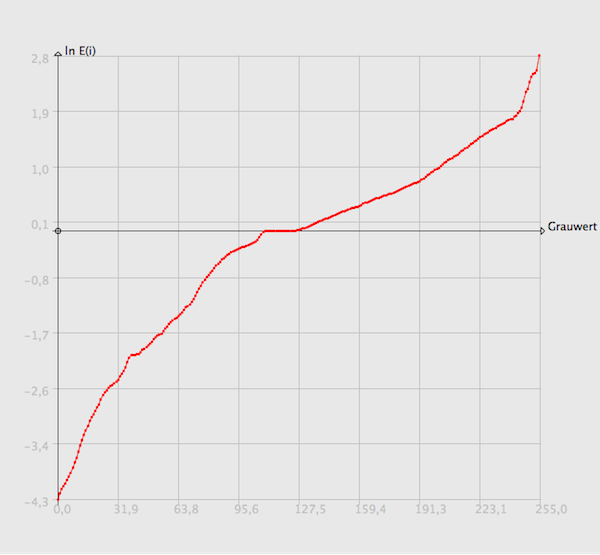
\includegraphics[width=0.45\textwidth]{sample_2/g_mon}
    \caption{\textbf{oben:} Belichtungsserie, Belichtungszeit: 1/8000, 1/640, 1/100 (v.l.), \textbf{u.l.:} Antwortkurve ohne Monotonie-Forderung, \textbf{u.r.:} Antwortkurve mit Monotonie-Forderung}
    \label{fig:mon:1}
  \end{center}
\end{figure}



\subsection{Ergebnisse mit räumlichem Glattheitsterm}

Die Erweiterung des räumlichen Glattheitsterms sorgt dafür, dass die benachbarten Pixel bei der Berechnung der \gls{Radiance Map} berücksichtigt werden. Wie in \autoref{fig:raum:1} zu sehen, hat dies insbesondere bei Messfehlern (hier 4\% \gls{SaltAndPepperNoise}) einen enormen Vorteil gegenüber dem herkömmlichen Verfahren. Auch durch Störungen wir das additive Gauss-Rauschen ($\sigma=10$, siehe \autoref{fig:raum:2}) sind die Ergebnisse schärfer und das Rauschen auf den Eingangsbildern wird reduziert.


\begin{figure}
  \begin{center}
    \begin{tikzpicture}[spy using outlines={circle,red,magnification=4,size=6cm, connect spies}]
        \node {
            \begin{overpic}[width=0.6\textwidth]{raum/E_ohne}
                \put(-0,0){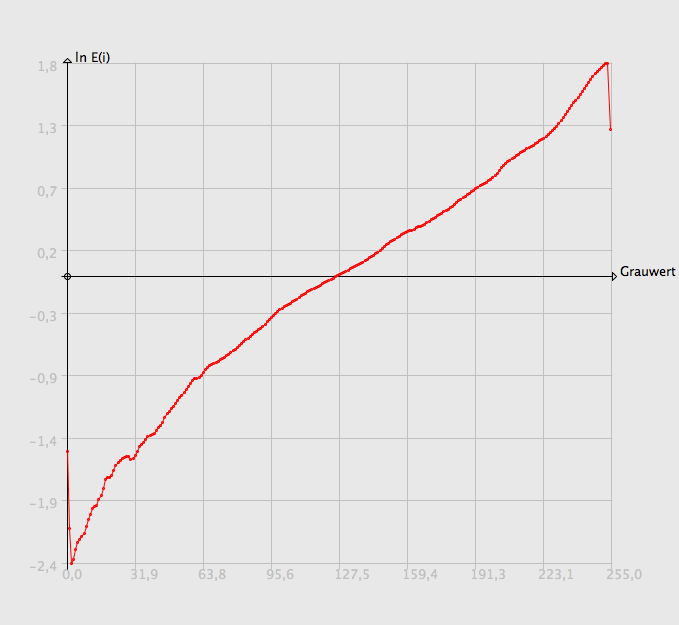
\includegraphics[width=3cm]{raum/g_ohne}}
            \end{overpic}
        };
        \spy on (1.8,-1.3) in node [left] at (9.5,0);
    \end{tikzpicture}
    
    \begin{tikzpicture}[spy using outlines={circle,red,magnification=4,size=6cm, connect spies}]
        \node {
            \begin{overpic}[width=0.6\textwidth]{raum/E_mit}
                \put(-0,0){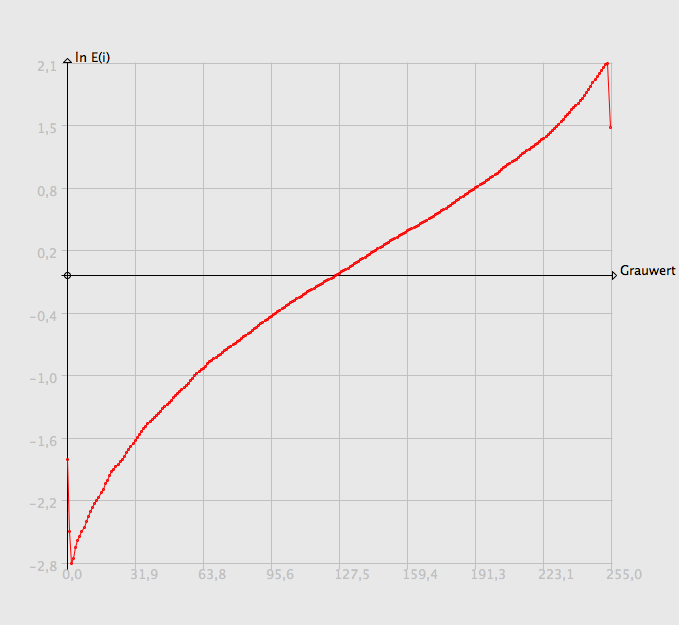
\includegraphics[width=3cm]{raum/g_mit}}
            \end{overpic}
        };
        \spy on (1.8,-1.3) in node [left] at (9.5,0);
    \end{tikzpicture}
    \caption{Einfluss des räumlichen Glattheitsterms auf verrauschte Bilder (4\% \gls{SaltAndPepperNoise}): \textbf{oben:} Antwortkurve und zugehöroges HDR Bild ohne räumlichen Glattheitsterm, \textbf{unten:} Antwortkurve mit räumlichem Glattheitsterm ($\alpha = 1$) und zugehöriges HDR-Bild. Das \gls{SaltAndPepperNoise} ist im unteren Bild quasi nicht mehr zu erkennen.}
    \label{fig:raum:1}
  \end{center}
\end{figure}

\begin{figure}
  \begin{center}
    \begin{tikzpicture}[spy using outlines={circle,red,magnification=4,size=6cm, connect spies}]
        \node {
            \begin{overpic}[width=0.6\textwidth]{raum/E_gauss_ohne}
                \put(-0,0){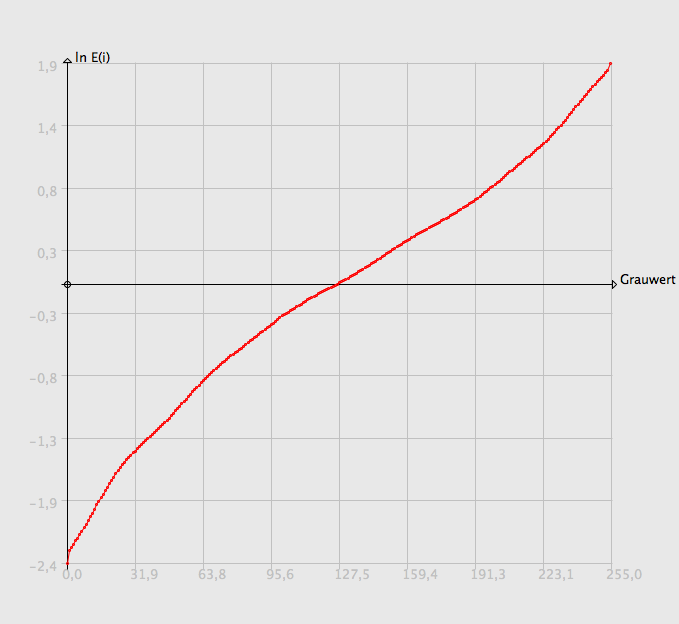
\includegraphics[width=3cm]{raum/g_gauss_ohne}}
            \end{overpic}
        };
        \spy on (1.8,-1.3) in node [left] at (9.5,0);
    \end{tikzpicture}
    
    \begin{tikzpicture}[spy using outlines={circle,red,magnification=4,size=6cm, connect spies}]
        \node {
            \begin{overpic}[width=0.6\textwidth]{raum/E_gauss_mit}
                \put(-0,0){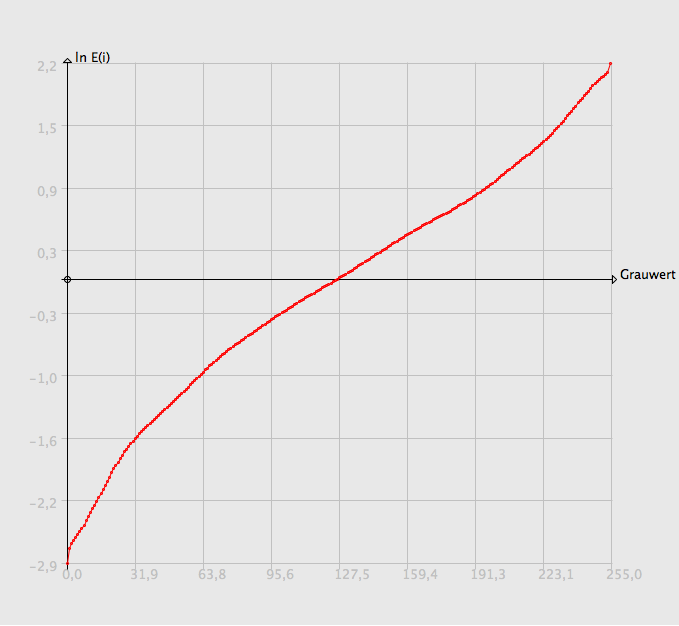
\includegraphics[width=3cm]{raum/g_gauss_mit}}
            \end{overpic}
        };
        \spy on (1.8,-1.3) in node [left] at (9.5,0);
    \end{tikzpicture}
    \caption{Einfluss des räumlichen Glattheitsterms auf verrauschte Bilder (additives Gauss-Rauschen mit $\sigma = 10$): \textbf{oben:} Antwortkurve und zugehöriges HDR Bild ohne räumlichen Glattheitsterm, \textbf{unten:} Antwortkurve mit räumlichem Glattheitsterm ($\alpha = 1$) und zugehöriges HDR-Bild.}
    \label{fig:raum:1}
  \end{center}
\end{figure}

\subsection{Ergebnisse mit Robustheits-Term}

Besonders die Erweiterung mit subquadratischen Bestrafungsfunktionen liefert eine Verbesserung des Standard Verfahrens. 


\begin{figure}
  \begin{center}
    \begin{tikzpicture}[spy using outlines={circle,red,magnification=4,size=6cm, connect spies}]
        \node {
            \begin{overpic}[width=0.6\textwidth]{results/E1}
                \put(-0,0){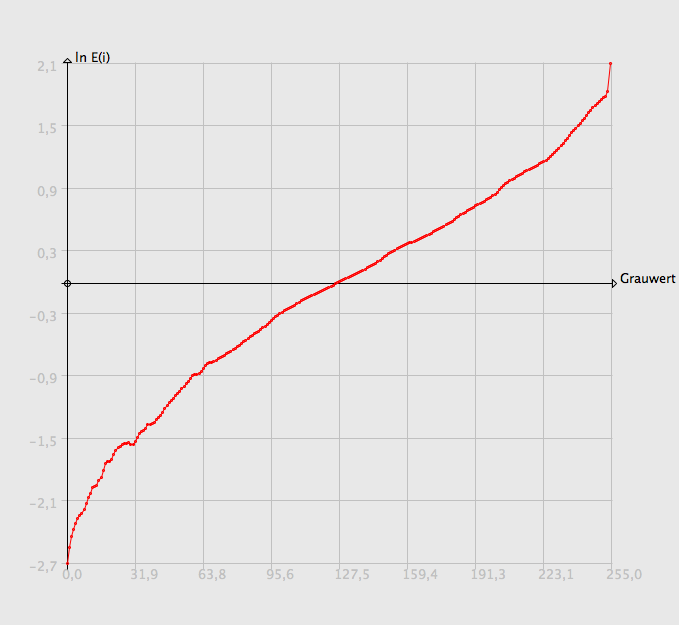
\includegraphics[width=3cm]{results/g1}}
            \end{overpic}
        };
        \spy on (1.8,-1.3) in node [left] at (9.5,0);
    \end{tikzpicture}
    
    \begin{tikzpicture}[spy using outlines={circle,red,magnification=4,size=6cm, connect spies}]
        \node {
            \begin{overpic}[width=0.6\textwidth]{raum/E_gauss_mit}
                \put(-0,0){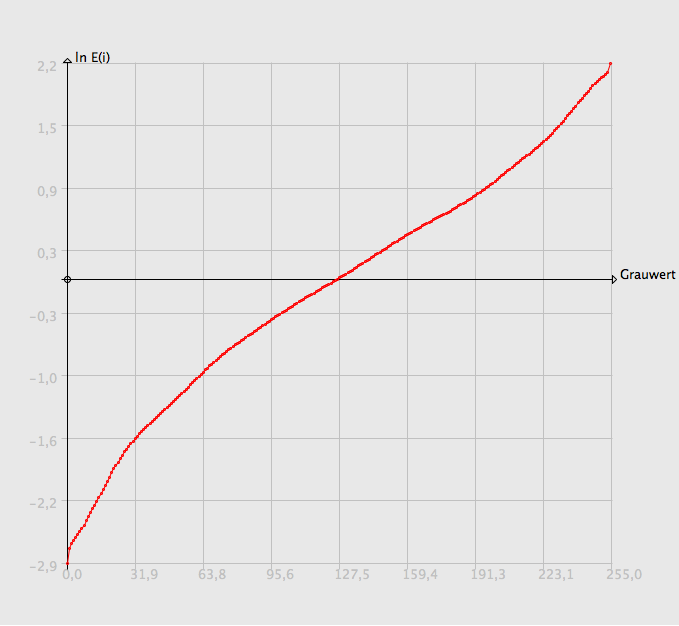
\includegraphics[width=3cm]{raum/g_gauss_mit}}
            \end{overpic}
        };
        \spy on (1.8,-1.3) in node [left] at (9.5,0);
    \end{tikzpicture}
    \caption{Einfluss der subquadratischen Bestrafungsfunktionen: \textbf{oben:} Standardverfahren, \textbf{unten:} Subquadratischer Bestrafungsterm $\varphi(s^2)=\sqrt{s^2+\epsilon^2}$}
    \label{fig:raum:1}
  \end{center}
\end{figure}
